% ================================================
% Please HIGHLIGHT the new inputs such like this :
% Text :
%  \hl{comment}
% Aligned Eq. 
% \begin{shaded}
% \end{shaded}
% ================================================



\documentclass[conference]{IEEEtran}

%\usepackage[retainorgcmds]{IEEEtrantools}
%\usepackage{bibentry}  
\usepackage{xcolor,soul,framed} %,caption

\colorlet{shadecolor}{yellow}
% \usepackage{color,soul}
\usepackage[pdftex]{graphicx}
\graphicspath{{../pdf/}{../jpeg/}}
\DeclareGraphicsExtensions{.pdf,.jpeg,.png}

\usepackage[cmex10]{amsmath}
%Mathabx do not work on ScribTex => Removed
%\usepackage{mathabx}
\usepackage{array}
\usepackage{mdwmath}
\usepackage{mdwtab}
\usepackage{eqparbox}
\usepackage{url}

\hyphenation{op-tical net-works semi-conduc-tor}

%\bstctlcite{IEEE:BSTcontrol}


%=== TITLE & AUTHORS ====================================================================
\begin{document}
\bstctlcite{IEEEexample:BSTcontrol}
    \title{Using Deep Inverse Reinforcement Learning to Learn the Social Force Model}
  \author{Yigit YILDIRIM,~\IEEEmembership{Student Member,~IEEE,}
      Irmak GUZEY,~\IEEEmembership{Student Member,~IEEE,}
      H. Levent AKIN~\IEEEmembership{Fellow,~IEEE}% <-this % stops a space

  \thanks{Manuscript received July 10, 2012. \hl{This paper is an expanded paper from the IEEE MTT-S Int. Microwave Symposium held on June 17-22, 2012 in Montreal, Canada.} This work was funded in part by the Office of Naval Research under the Defense Advanced Research Projects Agency (DARPA) Microscale Power Conversion (MPC) Program under Grant N00014-11-1-0931, and in part by the Advanced Research Projects Agency-Energy (ARPA-E), U.S. Department of Energy, under Award Number DE-AR0000216.}
  \thanks{M. Roberg is with TriQuint Semiconductor, 500 West Renner Road Richardson, TX 75080 USA (e-mail: michael.roberg@tqs.com).}% <-this % stops a space
  \thanks{T. Reveyrand is with the XLIM Laboratory, UMR 7252, University of Limoges, 87060 Limoges, France (e-mail: tibault.reveyrand@xlim.fr).}%
  \thanks{I. Ramos and Z. Popovic are with the Department of Electrical, Computer and Energy Engineering, University of Colorado, Boulder, CO, 80309-0425 USA (e-mail: ignacio.ramos@colorado.edu; zoya.popovic@colorado.edu).}% <-this % stops a space
  \thanks{E. Falkenstein is with Qualcomm Inc., 6150 Lookout Road
Boulder, CO 80301 USA (e-mail: erez.falkenstein@gmail.com).}}  


% The paper headers
\markboth{IEEE TRANSACTIONS ON MICROWAVE THEORY AND TECHNIQUES, VOL.~60, NO.~12, DECEMBER~2012
}{Roberg \MakeLowercase{\textit{et al.}}: High-Efficiency Diode and Transistor Rectifiers}


% ====================================================================
\maketitle



% === ABSTRACT ====================================================================
% =================================================================================
\begin{abstract}
%\boldmath
Abs
\end{abstract}


% === KEYWORDS ====================================================================
% =================================================================================
\begin{IEEEkeywords}
\hl{key0, key1}
\end{IEEEkeywords}


% For peer review papers, you can put extra information on the cover
% page as needed:
% \ifCLASSOPTIONpeerreview
% \begin{center} \bfseries EDICS Category: 3-BBND \end{center}
% \fi
%
% For peerreview papers, this IEEEtran command inserts a page break and
% creates the second title. It will be ignored for other modes.
\IEEEpeerreviewmaketitle


% ====================================================================
% ====================================================================
% ====================================================================











% === I. INTRODUCTION =============================================================
% =================================================================================
\section{Introduction}

Intro

% === II. Section 2 ========================
% =================================================================================
\section{Title}


% =======
% FIG. 01
% =======
\begin{figure}
  \begin{center}
  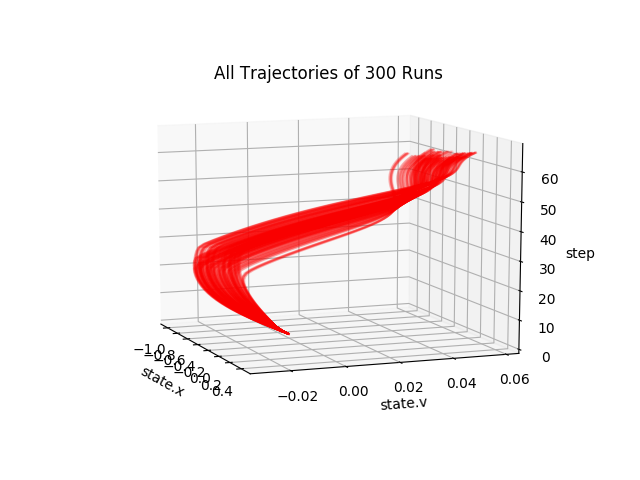
\includegraphics[width=3.5in]{img/0.png}
  \caption{Caption.}\label{circuit_diagram}
  \end{center}
\end{figure}

\begin{equation}\label{ideal_rectifier_resistance}
R(v) =
\begin{cases}
    \infty, & v > 0\\
    0, & v \leq 0
\end{cases}
\end{equation}
 Fig.~\ref{circuit_diagram} 

\subsection {Subs}

In Fig.~\ref{circuit_diagram}, given (\ref{ideal_rectifier_resistance}).


% === III. Sec3 =======================================
% =================================================================================
\section{Sec3}



% === IV. ========================================
% =================================================================================
\section{S4}

\subsection {Measurement setup}
Test

% === V. Bla ========================================
% =================================================================================
\section{S5}
S5 \cite{erezMTT2012}.


\section*{Acknowledgment}
We ack 


% Can use something like this to put references on a page
% by themselves when using endfloat and the captionsoff option.
\ifCLASSOPTIONcaptionsoff
  \newpage
\fi

\bibliographystyle{IEEEtran}
\bibliography{ref}

\vfill

% that's all folks
\end{document}
